%% language specific settings:
\lstdefinestyle{Arduino}{%
    language = Octave,
    keywords={void, int boolean},%                 define keywords
    morecomment=[l]{//},%             treat // as comments
    morecomment=[s]{/*}{*/},%         define /* ... */ comments
    emph={HIGH, OUTPUT, LOW}%        keywords to emphasize
}
\chapter{Układ pomiarowy do monitorowania saturacji krwi i fali tętna}
\section{Wprowadzenie do układu pomiarowego}
Układ ma na celu dostarczenie narzędzia do kompleksowego monitorowania parametrów fizjologicznych w czasie rzeczywistym takich jak saturacja krwi oraz fala tętna, umożliwiając jednocześnie mobilność i łatwość użytkowania. Dzięki temu badania z wykorzystaniem tego układu mogą dostarczyć cennych informacji na temat reakcji organizmu na różne bodźce oraz zmian w warunkach środowiskowych.
\begin{figure}[!htb]
    \centering
    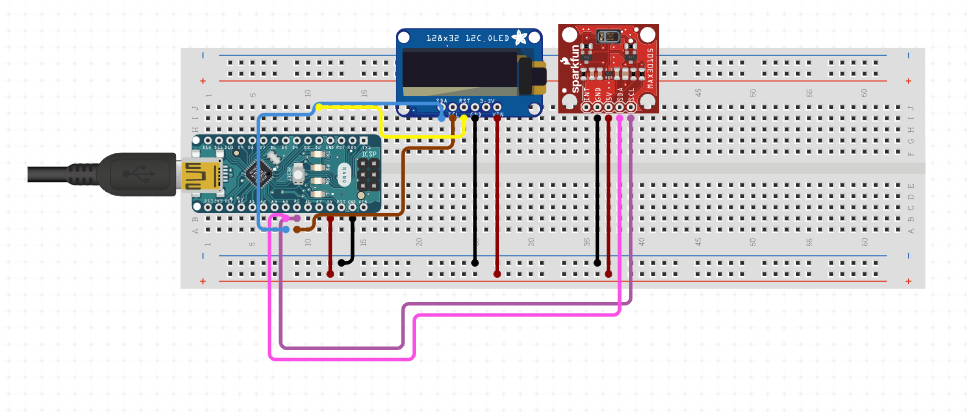
\includegraphics[width=.9\linewidth]{uklad_pogladowy.png}
    \caption{Układ poglądowy wykonany na stronie \textit{www.circuito.io}}
\end{figure}

Układ został celowo zaprojektowany w minimalistycznym stylu, aby umożliwić wygodne przymocowanie do rękawiczki, którą nosi osoba badana. Jego kompaktowa forma i lekka konstrukcja pozwalają na swobodne użytkowanie, minimalizując jednocześnie wpływ na naturalne ruchy i komfort badanego. Wszystkie wykorzystane technologie, takie jak mikrokontroler Arduino Nano, czujnik pulsoksymetryczny MAX30102, czy wyświetlacz OLED 128x64, zostały dokładnie opisane w poprzednich sekcjach. Dzięki takiemu podejściu, układ spełnia funkcję efektywnego narzędzia do zbierania danych fizjologicznych, zachowując jednocześnie prostotę i praktyczność w użyciu.

\section{Wykorzystane technologie}
Stworzony został kompleksowy układ pomiarowy, umożliwiający zbieranie danych dotyczących czasu reakcji, saturacji krwi i fali tętna. Poniżej przedstawiono szczegółowy opis implementacji poszczególnych komponentów układu:
\subsection{Komponenty fizyczne}
\begin{itemize}
  \item Mikrokontroler Arduino Nano: Układ sterujący oparty na mikrokontrolerze Arduino Nano, charakteryzującym się kompaktowym designem i wysoką wydajnością. Odpowiada za odbiór danych z czujnika MAX30102, ich efektywne przetwarzanie oraz kontrolę wyświetlacza OLED
  \begin{figure}[!htb]
    \centering
    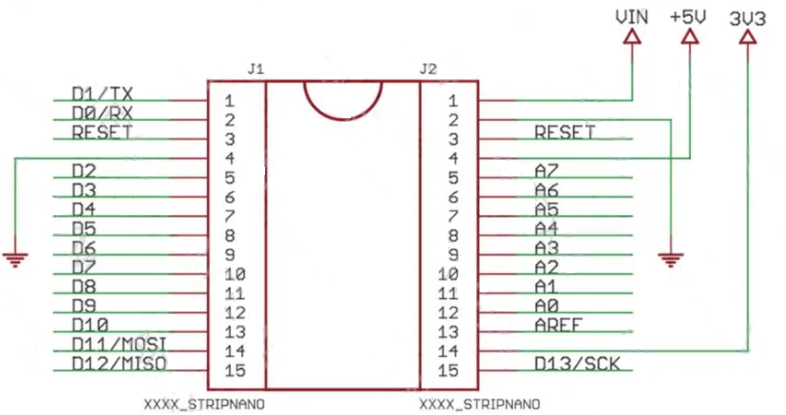
\includegraphics[width=.7\linewidth]{arduino.png}
    \caption{Konfiguracja pinów mikrokontrolera w ofercie sprzedaży dostawcy \cite{arduinofota}}
  \end{figure}
  \item Czujnik Pulsoksymetryczny MAX30102: Centralny element pomiarowy oparty na czujniku MAX30102, specjalnie zaprojektowanym do precyzyjnych pomiarów saturacji krwi i fali tętna. Zlokalizowany na palcu, co umożliwia bezpośrednie i komfortowe zbieranie danych dotyczących parametrów fizjologicznych.
  \begin{figure}[!htb]
    \centering
    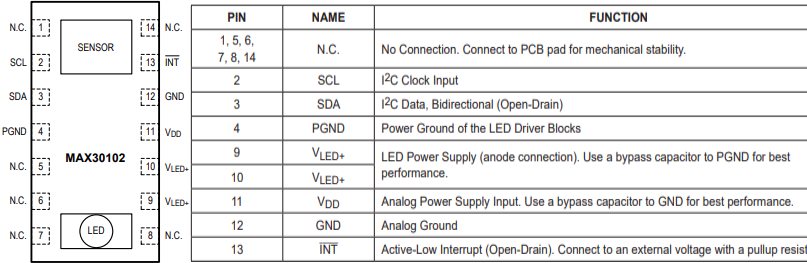
\includegraphics[width=.7\linewidth]{max30102.png}
    \caption{Konfiguracja oraz opis pinów w czujniku MAX30102 \cite{max30102}}
  \end{figure}
  \item Wyświetlacz OLED 128x64: Wykorzystano wyświetlacz OLED o rozdzielczości 128x32 pikseli do wizualizacji wyników pomiarów. Zapewnia intuicyjne prezentowanie informacji na bieżąco, co ma kluczowe znaczenie zarówno dla użytkownika, jak i podczas procesu kalibracji układu.
\end{itemize}

\begin{figure}[!htb]
  \centering
  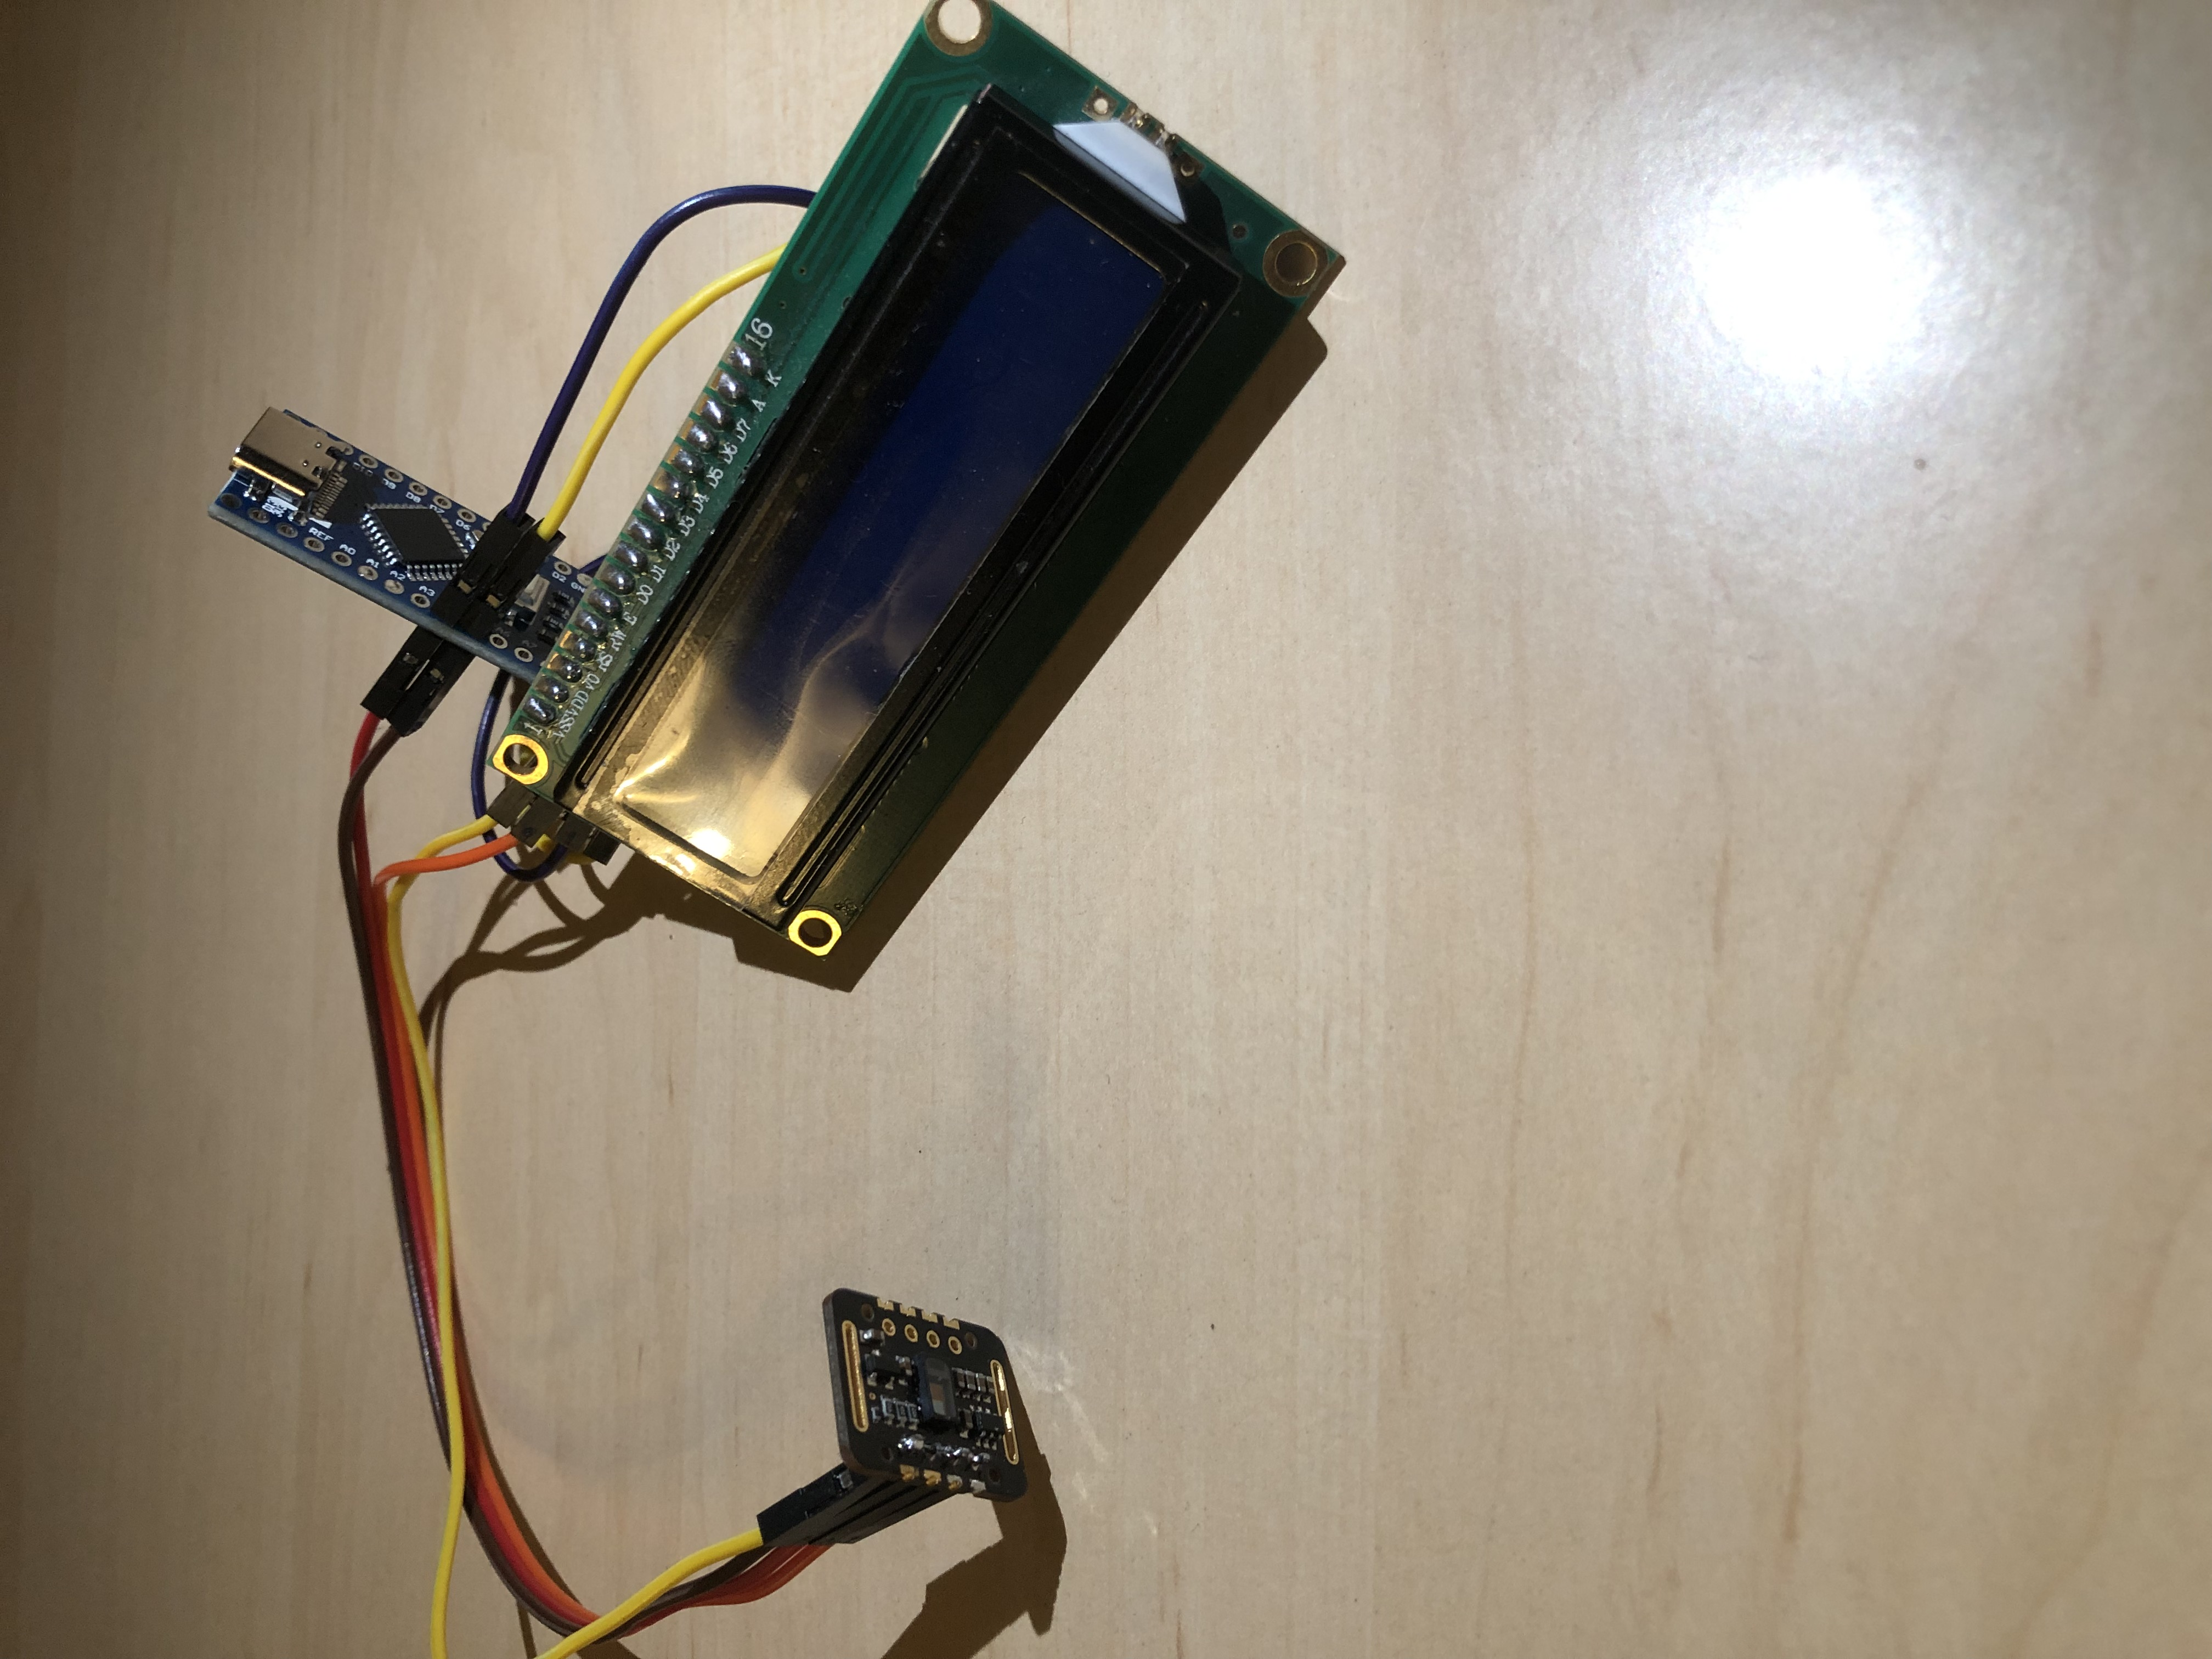
\includegraphics[width=.7\linewidth]{uklad1.jpg}
  \caption{Układ Arduino z modułem pulsoksymetru}
\end{figure}
\subsection{Aspekty programistyczne}
\begin{itemize}
  \item Arduino IDE: W projekcie wykorzystano środowisko programistyczne Arduino IDE, specjalnie zaprojektowane do programowania mikrokontrolerów Arduino \cite{arduino}. To narzędzie oferuje prosty interfejs użytkownika oraz zestaw bibliotek umożliwiających programowanie układów mikroprocesorowych.
  \item Język Programowania C++: Do programowania mikrokontrolera Arduino Nano użyto języka programowania C++. Język ten jest powszechnie stosowany w programowaniu mikrokontrolerów i zapewnia efektywną kontrolę nad działaniem układów. Dzięki zastosowaniu Arduino IDE i języka C++, udało się precyzyjnie sterować procesami pomiarowymi, co miało kluczowe znaczenie dla uzyskania wysokiej jakości danych pomiarowych.
  \item Biblioteki: Obydwa wykorzystane fragmenty kodu zostały zmodyfikowane i dostosowane w kontekście pracy inżynierskiej, wykorzystując dostępną publicznie bibliotekę \lstinline[language=C,basicstyle=\ttfamily]{SparkFun_MAX3010x_Pulse_and_Proximity_Sensor_Library}.
\end{itemize}

\section{Montaż układu}
Główna część układu została starannie umieszczona w pudełku wydrukowanym przy użyciu drukarki 3D VORON 0.1. Projekt obudowy został stworzony za pomocą zaawansowanej aplikacji Fusion 360. Projekcja pudełka uwzględniała ergonomiczne wymiary, a także precyzyjnie zaplanowane otwory, mające spełniać różnorodne funkcje. W trakcie projektowania uwzględniono otwór umożliwiający obserwację wyników pomiarów na wyświetlaczu OLED, co pozwala użytkownikowi na monitorowanie danych w czasie rzeczywistym. Dodatkowo przewidziano otwory na zamocowanie poszczególnych komponentów, takie jak miejsce na odprowadzenie kabli czy otwór umożliwiający podpięcie płytki do komputera w celu konfiguracji czy aktualizacji oprogramowania. 
\begin{figure}[!htb]
  \centering
  \includegraphics[width=.7\linewidth]{pudełko1.png}
  \caption{Rysunek techniczny większego pudełka wykonany w programie AutoCAD}
\end{figure}
Dla zabezpieczenia czujnika przed uszkodzeniem, specjalnie zaprojektowano i wydrukowano pudełko, które skutecznie ochrania ten kluczowy element układu. Projekt pudełka dla czujnika został dostosowany do jego kształtu i wymiarów, zapewniając idealne dopasowanie oraz ochronę przed ewentualnymi uszkodzeniami mechanicznymi. Takie staranne podejście do projektowania obudowy gwarantuje nie tylko estetyczny wygląd układu, ale także funkcjonalność oraz łatwość obsługi. Otwory i szczegóły konstrukcyjne zostały dokładnie dostosowane do potrzeb użytkownika, zapewniając jednocześnie trwałość i ochronę komponentów.
\begin{figure}[!htb]
  \centering
  \includegraphics[width=.8\linewidth]{pudełko2.png}
  \caption{Rysunek techniczny mniejszego pudełka wykonany w programie AutoCAD}
\end{figure}
Całość układu została solidnie zamocowana na rękawiczce, co zapewnia stabilność i wygodę noszenia przez osobę badaną. Przewody zostały starannie odprowadzone i zabezpieczone, umożliwiając jednocześnie przypięcie czujnika do palca. Zaizolowane kable gwarantują nie tylko bezpieczne połączenia elektryczne, ale także komfort użytkowania oraz ochronę przed ewentualnymi zakłóceniami zewnętrznymi.
\begin{figure}[!htb]
  \centering
  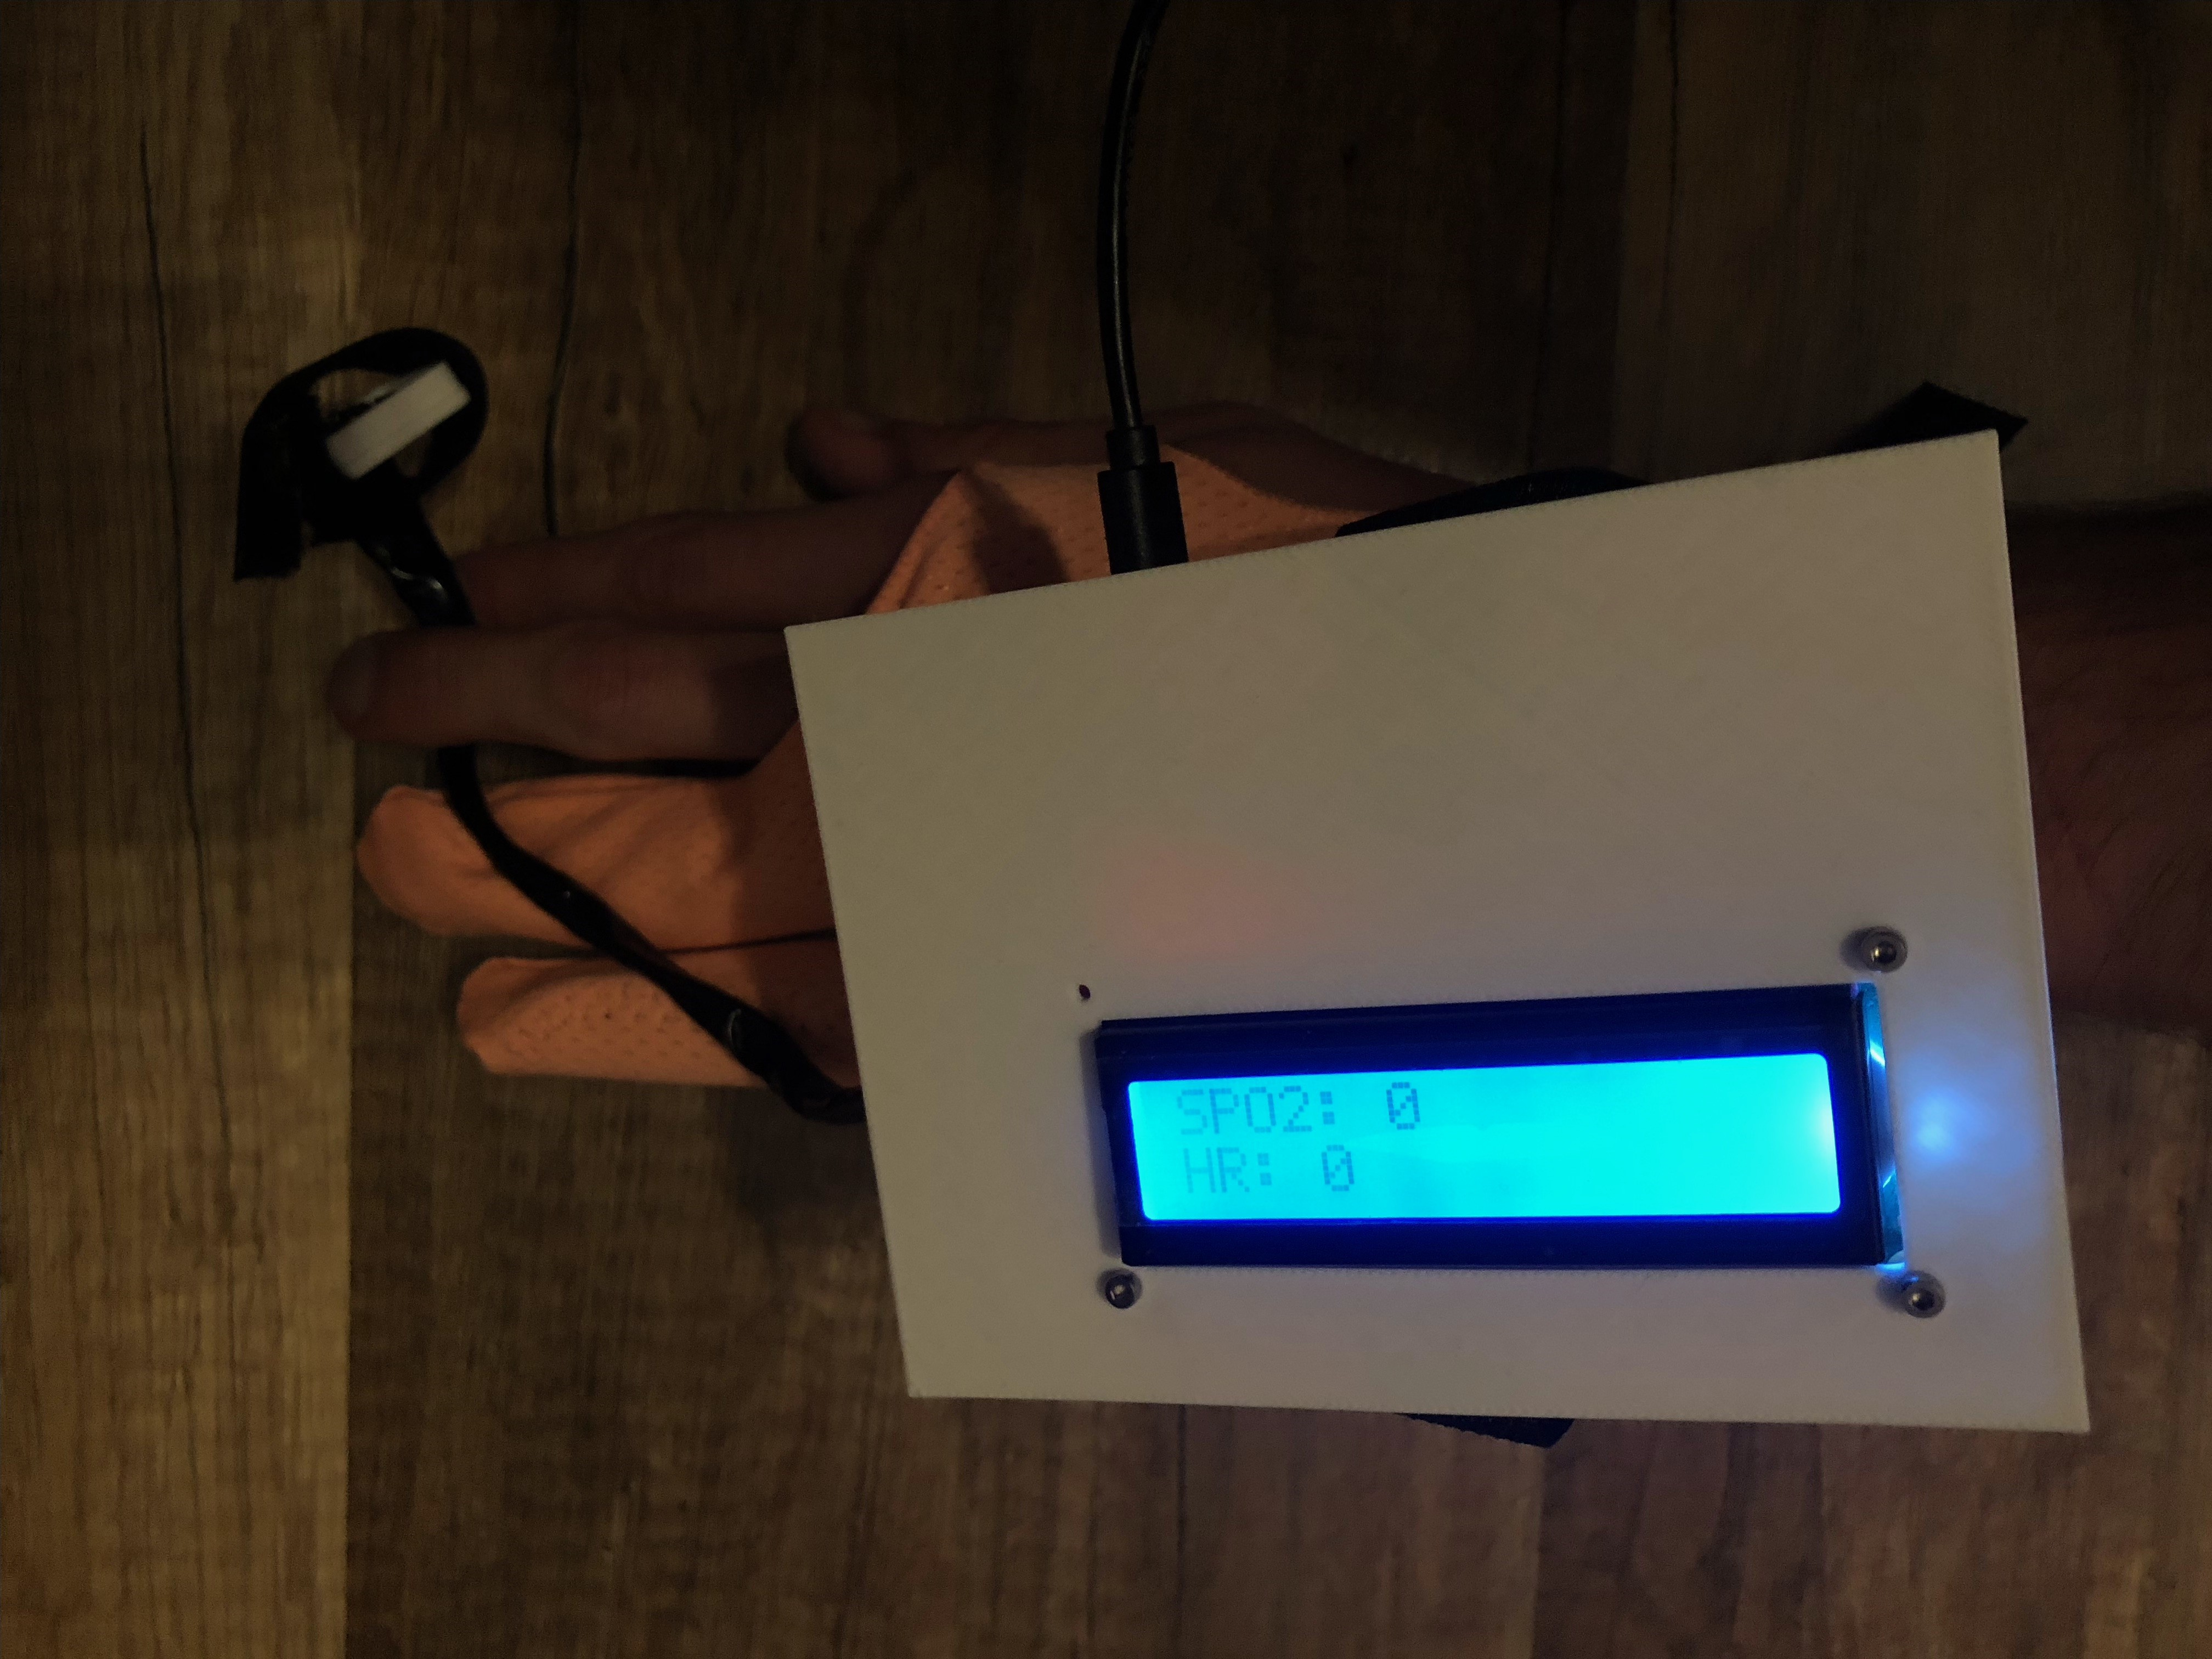
\includegraphics[width=.8\linewidth]{ukladkoncowy.jpeg}
  \caption{Układ pomiarowy zamontowany na rękawicze}
\end{figure}

